\section{Auswertung}
\label{sec:Auswertung}
Die Funktionsweise des Versuchsaufbaus mit dem Vorgehen nach Abschnitt \ref{sec:durchfuehrung_1} wurde getestet
und die Messung gestartet, 
nachdem das System ausreichend aufgeheizt ist.

Die Amplitude $A$ ist ein Maß für die Leistung $P$ und wird in willkürlichen Einheiten oder Skalenteile gemessen,
da Berechnung nur bei Leistungsverhältnisse stattfinden.
%
\subsection{Untersuchung der Moden des Reflexklystrons}
%
\begin{table}
\centering
\caption{Messwerte zur Untersuchung der Moden des Reflexklystrons.}
\begin{tabular}{c cccccc}
	\toprule
	{\# Mode} &$\frac{U_-}{\si{\volt}}$ &$\frac{U_\text{max}}{\si{\volt}}$ &$\frac{U_+}{\si{\volt}}$ &$A_\text{Messung}$ &$A_\text{Fit}$ &$\frac{f_0}{\si{\giga\hertz}}$\\
	\midrule
		1 &200 	&220 &230 	&6.3 &7.087 &9.000 \\
		2 &120 	&140 &150 	&6.3 &7.087 &9.003 \\
		3 &70 	& 80 &90 	&5.3 &5.3 &9.010 \\
	\bottomrule
\end{tabular}
\label{tab:moden}
\end{table}

Die Moden des Reflexklystrons können bestimmt werden,
indem die Reflektorspannungen $U_-$, $U_\text{max}$, $U_+$ und die Amplitude $A$ aufgenommen werden, 
bei welchen ein Oszillogram nach Abbildung \ref{fig:moden} angezeigt wird.
Die Frequenz $f_0$ wird bestimmt, indem der Frequenzmesser so eingestellt wird, sodass exakt die Spitze der Mode in Abbildung \ref{fig:moden} geringfügig eindellt.
Die Messwerte sind in Tabelle \ref{tab:moden} dargestellt und werden in Abbildung \ref{plt:moden} als Messpunkte und Fit einer quadratischen Funktion 
%
\begin{equation}
	P(U)= a\cdot x^2 + b\cdot x + c
	\label{eq:quadfkt}
\end{equation}
%
aufgetragen.
In dieser Abbildung sind die Messpunkte bei den beiden größten Moden nicht an dem Hochpunkt der Modenkurve, 
da die Spannungen $U_\pm$ nicht symmetrisch um das Maximum liegen.
Dies ist auf zu geringe Ablesbarkeit des Voltmeters für die Reflektorspannung zurückzuführen und stellt eine Fehlerquelle dar.
\begin{figure}
  \centering
  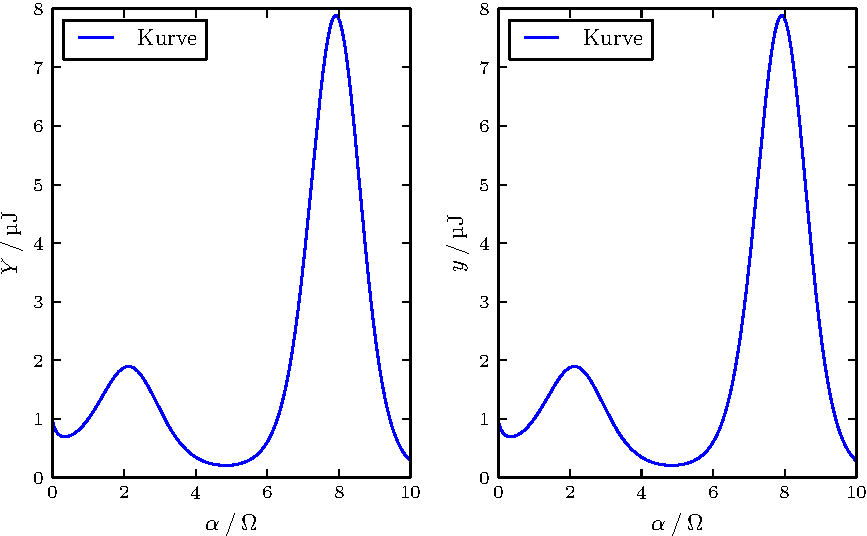
\includegraphics[width=\textwidth]{pc/plot.pdf}
  \caption{Darstellung der gemessenen Moden des Reflexklystrons.}
  \label{plt:moden}
\end{figure}

%
\begin{table}
\centering
\caption{Messwerte für die elektronische Abstimmung.}
\begin{tabular}{c cc}
	\toprule
	&{untere Grenze} &{obere Grenze}\\
	\midrule
		{Spannung/$\si{\volt}$} &210 &230 \\
		{Frequenz/$\si{\mega\hertz}$} &8978 &9023\\
	\bottomrule
\end{tabular}
\label{tab:elktr_abstimmung}
\end{table}
%
Die elektronische Abstimmung benötigt, gemessen an der größtmöglichen Mode, die Spannungen $U_{-\sfrac{1}{2}}$, $U_{\sfrac{1}{2}}$ und die dazugehörigen Frequenzen $f_{-\sfrac{1}{2}}$, $f_{\sfrac{1}{2}}$ bei halber Leistung.
Die Abstimmung ist durch
\begin{equation}
	A=\frac{f_{\sfrac{1}{2}}-f_{-\sfrac{1}{2}}}{U_{\sfrac{1}{2}}-U_{-\sfrac{1}{2}}} = \SI{2.25}{\mega\hertz\per\volt}
\end{equation}
gegeben;
Messwerte sind in Tabelle \ref{tab:elktr_abstimmung} aufgezählt.

\subsection{Untersuchung von Frequenz, Wellenlänge und Dämpfung}
Zur Berechnung der Wellenlänge 
\begin{equation}
	\lambda_\text c = 2a
\end{equation} 
werden die Abmessungen des Hohlleiters, im Detail die längere Innenseite $a$ des Leiterquerschnitts (vgl. Abb. \ref{fig:hohlleitung}), benötigt. 
Mit der Hohlleiter-Wellenlänge $\lambda_\text g$ als zweifachen Abstand zweier Intensitätsminima wird die Frequenz 
\begin{equation}
	f=c\sqrt{\frac{1}{\lambda^2_\text g}+\frac{1}{4a^2}}
\end{equation}
bestimmt und als Grundlage für die Dämpfungsmessung benützt.
Die Abmessungen, die Wellenlänge $\lambda_\text g$ und Frequenz $f$ sind in Tabelle \ref{tab:flambdagamma}
gezeigt. 
\begin{table}
\centering
\caption{Messwerte zur Untersuchung der Dämpfung.}
\begin{tabular}{ccccc}
	\toprule
	$\frac{f_\text{Messung}}{\si{\mega\hertz}}$& \
	$\frac{\symup{\Delta}x_\text{Minima}}{\si{\milli\meter}}$& \
	$\frac{a}{\si{\milli\meter}}$& \
	$\frac{\lambda_\text g}{\si{\milli\meter}}$& \
	$\frac{f_\text{Berechnung}}{\si{\mega\hertz}}$\\
	\midrule
		9023&	24.1&	22.62&	48.2&	9088.4\\
	\bottomrule
\end{tabular}
\label{tab:flambdagamma}
\end{table}

Tabelle \ref{tab:SWR_Daempfung} sind die Messwerte des SWR-Messer aufgetragten.
Zusätzlich zeigt es zum Messwert gehörende die Millimetereinstellung des Dämpfers und den zur Millimetereinstellung gehörende Theoriewert sowie die Abweichung zwischen Theoriewert und Messung.
Die Ergebnisse sind in Abbildung \ref{plt:daempfung} aufgetragen.
\begin{figure}
\centering
\includegraphics[width=0.9\textwidth]{pc/daempfung.pdf}
\caption{Graphische Darstellung der Dämpfung, Theorie und Messwerte.}
\label{plt:daempfung}
\end{figure}
\begin{table}
\centering
\caption{Gemessene und theoretische Dämpfung.}
\begin{tabular}{cccc}
	\toprule
	Messwert& \
	Dämpfereinstellung& \
	Theoriewert& \
	Abweichung \\
	$\si{\decibel}$& \
	$\si{\milli\meter}$& \
	$\si{\decibel}$& \
	\%\\
	\midrule
		2&  1,345&   3,64&-98\\
		4&  1,698&   5,65&-96\\
		6&  2,115&   8,59&-94\\
		8&  2,341&  10,43&-92\\
		10& 2,609&  12,86&-90\\
	\bottomrule
\end{tabular}
\label{tab:SWR_Daempfung}
\end{table}

\subsection{Untersuchung von stehenden Wellen}
Die stehenden Wellen werden mit drei Methoden -- SWR-Methode, $\SI{3}{\decibel}$-Methode,Abschwächermethode -- ausgemessen. 
Die Ergebnisse der SWR-Methode sind in Tabelle \ref{tab:swr_methode}, die Ergenisse der $\SI{3}{\decibel}$-Methode in Tabelle \ref{tab:3dB} und die Ergebnisse der Abschwächer-Methode in Tabelle \ref{tab:Abschwaecher} aufgelistet.
Zur Bestimmung der Stehwellenverhältnisse wurden in der SWR-Methode die Ausgabe des Messgerätes ausgelesen, bei den anderen Methoden wurden die Formeln
\begin{align}
	S_\text{3dB}&=\sqrt{1+\frac{1}{\sin²\left(\frac{\pi(d_2-d_1)}{\lambda_\text g}\right)}}\\
	S_\text{Abschwächer}&=\frac{\symup\Delta A}{2}
\end{align}
mit dem doppelten Abstand zweier Minima $\lambda_\text g$ benutzt.
\begin{table}
\centering
\caption{Ergebnisse der SWR-Methode.}
\begin{tabular}{cc}
	\toprule
	Tiefe der Nadel& SWR-Messwert\\
	\si{\milli\meter}& a.u.\\
	\midrule
	3& 1,1\\
	5& 1,5\\
	7& 2,8\\
	8& 4\\
	9& \infty \\
	\bottomrule
\end{tabular}
\label{tab:swr_methode}
\end{table}
\begin{table}
\centering
\caption{Ergebnisse der $\SI{3}{\decibel}$-Methode.}
\begin{tabular}{cccccc}
	\toprule
	$\frac{d_1}{\si{\milli\meter}}$& \
	$\frac{d_2}{\si{\milli\meter}}$& \
	$\frac{\text{1.Min}}{\si{\milli\meter}}$& \
	$\frac{\text{2.Min}}{\si{\milli\meter}}$& \
	$\frac{\lambda_\text g}{\si{\milli\meter}}$& \
	$\frac{S}{\si{\decibel}}$\\
	\midrule
	78,8&	92,7&	5&	33& 56&	2,37\\
	\bottomrule
\end{tabular}
\label{tab:3dB}
\end{table}
\begin{table}
\centering
\caption{Ergebnisse der Abschwächer-Methode.}
\begin{tabular}{cccc}
	\toprule
	$\frac{A_1}{\si{\decibel}}$& \
	$\frac{A_2}{\si{\decibel}}$& \	
	$\frac{\symup\Delta A}{\si{\decibel}}$& \	
	$\frac{S}{\si{\decibel}}$\\
	\midrule
	20&	38&	18&	9\\
	\bottomrule
\end{tabular}
\label{tab:Abschwaecher}
\end{table}